\section{Trigonometrische Funktionen (115-126)}
 
Sie brauchen NICHT die Potenzreihendefinition von Sinus und Kosinus auswendig wissen, sondern nur jeweils den schon aus der Schule bekannten groben Verlauf des reellen Sinus und des reellen Kosinus (also im Wesentlichen die Grafen mit Lage der Nullstellen, Maxima, Minima und Monotoniebereichen sowie sin*sin+cos*cos=1 - das beeinhaltet die Eigenschaften aus Th. 8.22 außer den Additionstheoremen und den Grenzwerten). Sie sollten auch wissen, dass sin und cos auf den ganzen komplexen Zahlen definiert und stetig sind. Eulersche Formel (8.46a). Definition von Tangens und Cotangens, ebenfalls mit Nullstellen und Monotonieintervallen. Polarkoordinaten komplexer Zahlen (Betrag,Argument). Darstellung in der komplexen Ebene. Multiplikation komplexer Zahlen in Polarkoordinaten. 

\subsection{reeller Sinus, reeller Cosinus}
\begin{figure}[H]
	\centering
  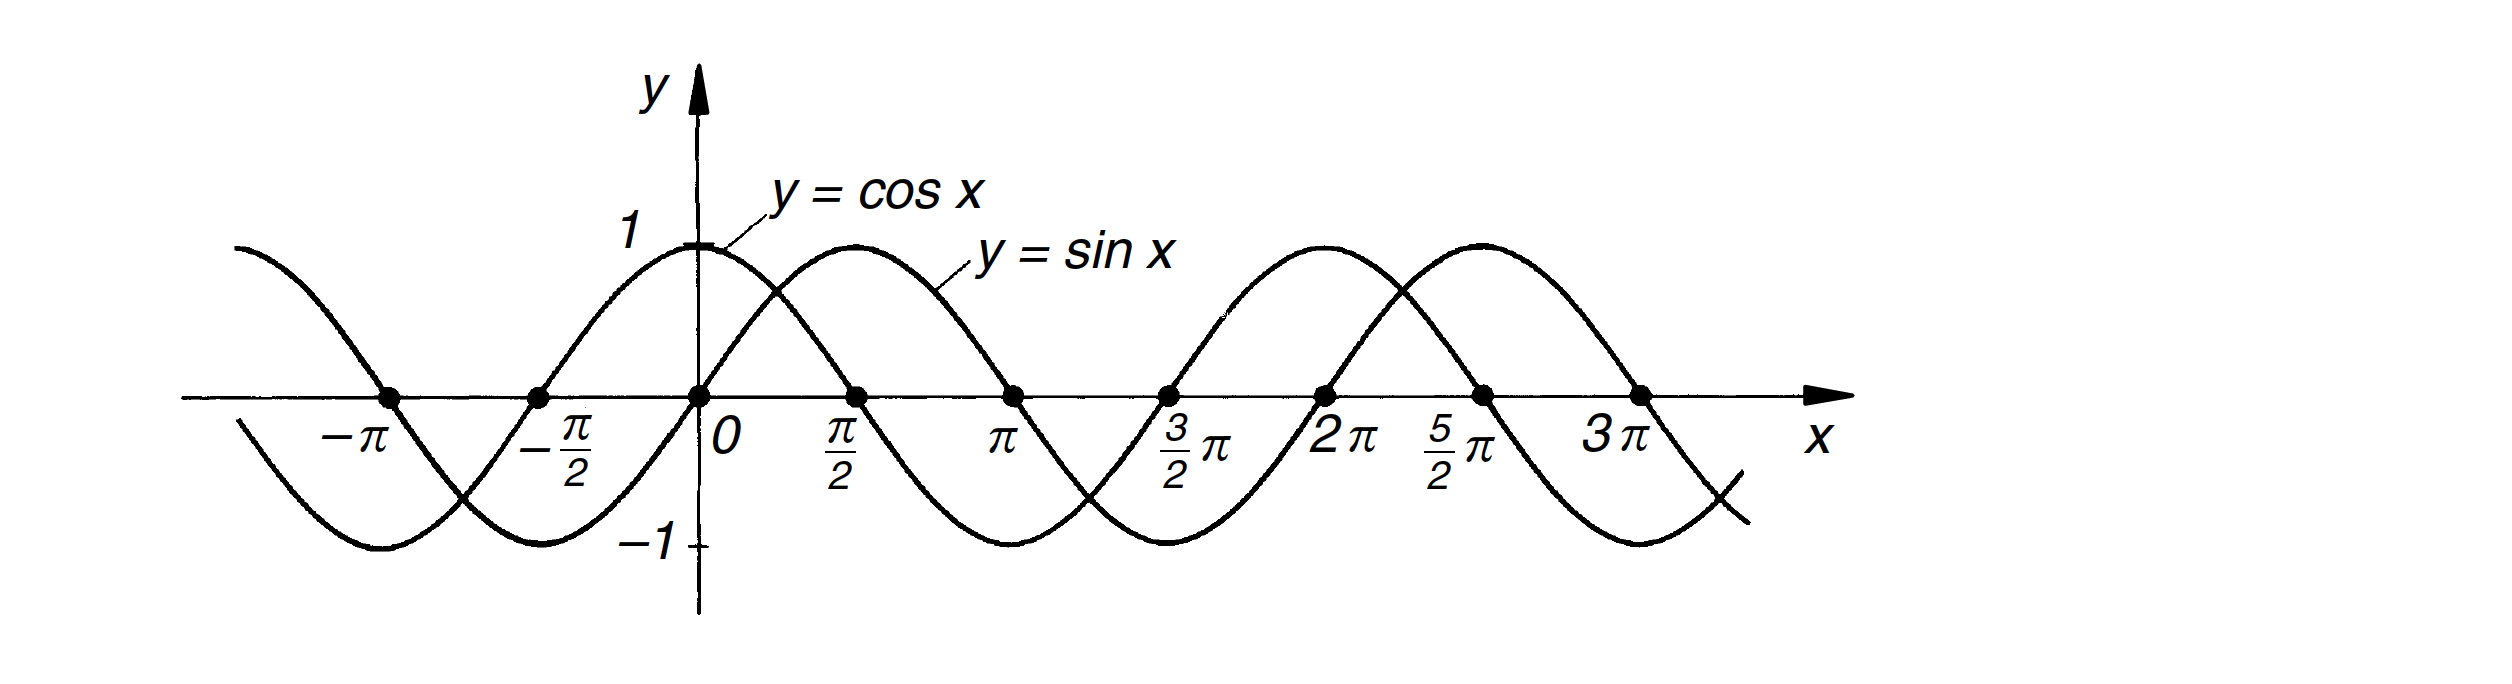
\includegraphics[width=\linewidth]{media/sin-cos.png}
	\caption{sin-cos}
	\label{sin-cos}
\end{figure}

\begin{table}[H]
%\centering
\begin{tabular}{|l||l|l|}
\hline
Eigenschaften ( $k \in \mathbb { Z }$ )     & $y= sin x$ & $y = cos x$ \\ \hline \hline
Definitionsbereich &     $- \infty < x < \infty$     &    $- \infty < x < \infty$       \\
Wertebereich       &    $ - 1\leq y \leq 1 $    &     $- 1\leq y \leq 1   $   \\ 
Periode (primitive)           &     $ 2\pi $   &    $ 2\pi  $    \\ 
Symmetrie          &     ungerade     &     gerade      \\ 
Nullstellen        &     $x _ { k } = k \cdot \pi$     &     $x _ { k } = \frac { \pi } { 2} + k \cdot \pi$      \\ 
Relative Maxima    &    $x _ { k } = \frac { \pi } { 2} + k \cdot 2\pi$      &      $x _ { k } = k \cdot 2\pi$     \\
Relative Minima    &     $x _ { k } = \frac { 3} { 2} \pi + k \cdot 2\pi$     &    $x _ { k } = \pi + k \cdot 2\pi$       \\ \hline
\end{tabular}
\caption{sin-cos-tab}
\label{sin-cos-tab}
\end{table}

Theorem 8.22
\begin{equation}
sin 0 = 0, \qquad cos 0 = 1
\end{equation}
\begin{equation}
\forall _ { z \in \mathbb { C } } \qquad\sin z = - \sin ( - z ) ,\qquad \cos z = \cos ( - z )
\end{equation}
\begin{equation}
\forall _ { z \in \mathbb { C } }  \qquad( \sin z ) ^ { 2} + ( \cos z ) ^ { 2} = 1
\end{equation}
\begin{equation}
\cos \frac { \pi } { 2} = 0,\quad \sin \frac { \pi } { 2} = 1,\quad \forall _ { x \in [ 0,\frac { \pi } { 2} } ] \cos x > 0
\end{equation}

\subsection{sin und cos sind auf den ganzen komplexen Zahlen definiert und stetig}

\subsection{Eulersche Formel (120)}
\begin{equation}
\underset{ z \in \mathbb { C } }{\forall} e ^ { i z } = \cos z + i \sin z
\end{equation}

\subsection{reeller Tangens, reeller Kotangens}
\begin{figure}[H]
	\centering
  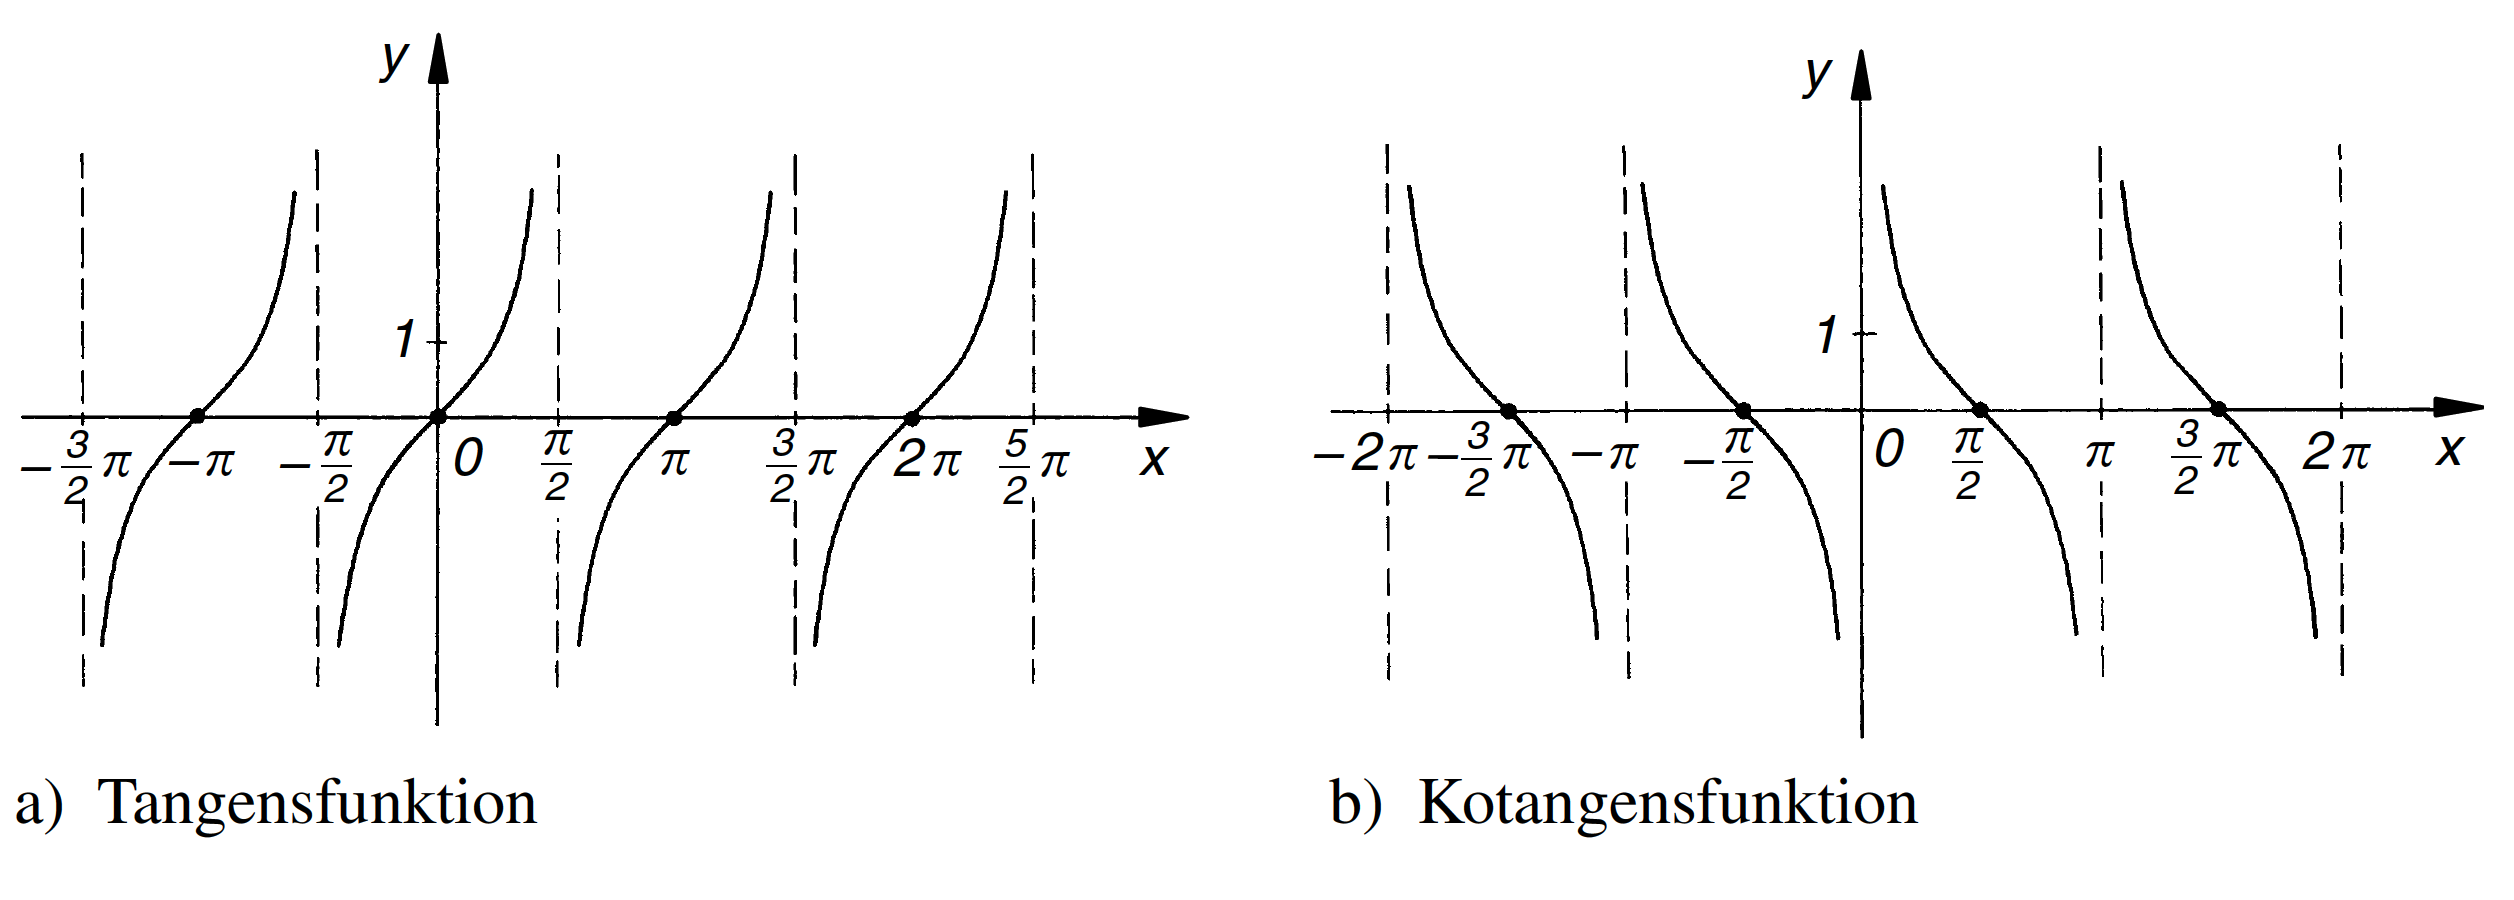
\includegraphics[width=\linewidth]{media/tan-cotan.png}
	\caption{tan-cotan}
	\label{tan-cotan}
\end{figure}

\begin{table}[H]
%\centering
\begin{tabular}{|l|l|l|}
\hline
Eigenschaften    ( $k \in \mathbb { Z }$ )     & $y= tan x$ & $y= cot x$ \\ \hline \hline
Definitionsbereich    &    \parbox[t]{2in}{ $x \in \mathbb { R }$ mit Ausnahme der Stellen \par  $x _ { k } = \frac { \pi } { 2} + k \cdot \pi$   }  &   \parbox[t]{2in}{   $x \in \mathbb { R }$ mit Ausnahme der Stellen  \par  $x _ { k } =  k \cdot \pi$   }    \\ 
Wertebereich          &   $- \infty < y < \infty$       &  $- \infty < y < \infty$          \\ 
Periode (primitive)   &   $\pi$       &      $\pi$     \\ 
Symmetrie             &    ungerade      &  ungerade         \\ 
Nullstellen           &     $x _ { k } = k \cdot \pi$     &      $x _ { k } = \frac { \pi } { 2} + k \cdot \pi$     \\ 
Pole                  &    $x _ { k } = \frac { \pi } { 2} + k \cdot \pi$      &    $x _ { k } = k \cdot \pi$       \\ 
Senkrechte Asymptoten &    $x = \frac { \pi } { 2} + k \cdot \pi$      &      $x = k \cdot \pi$        \\ \hline
\end{tabular}
\caption{tan-cotan-tab}
\label{tan-cotan-tab}
\end{table}

\begin{leftbar}
\noindent\begin{minipage}{.5\linewidth}
\begin{equation}
\tan x = \frac { \sin x } { \cos x } = \frac { 1} { \cot x }
\end{equation}
\end{minipage}
\begin{minipage}{.5\linewidth}
\begin{equation}
\cot x = \frac { \cos x } { \sin x } = \frac { 1} { \tan x }
\end{equation}
\end{minipage}
\end{leftbar}

\subsection{Polarkoordinaten komplexer Zahlen (Betrag, Argument) (123)}

\begin{figure}[H] \centering
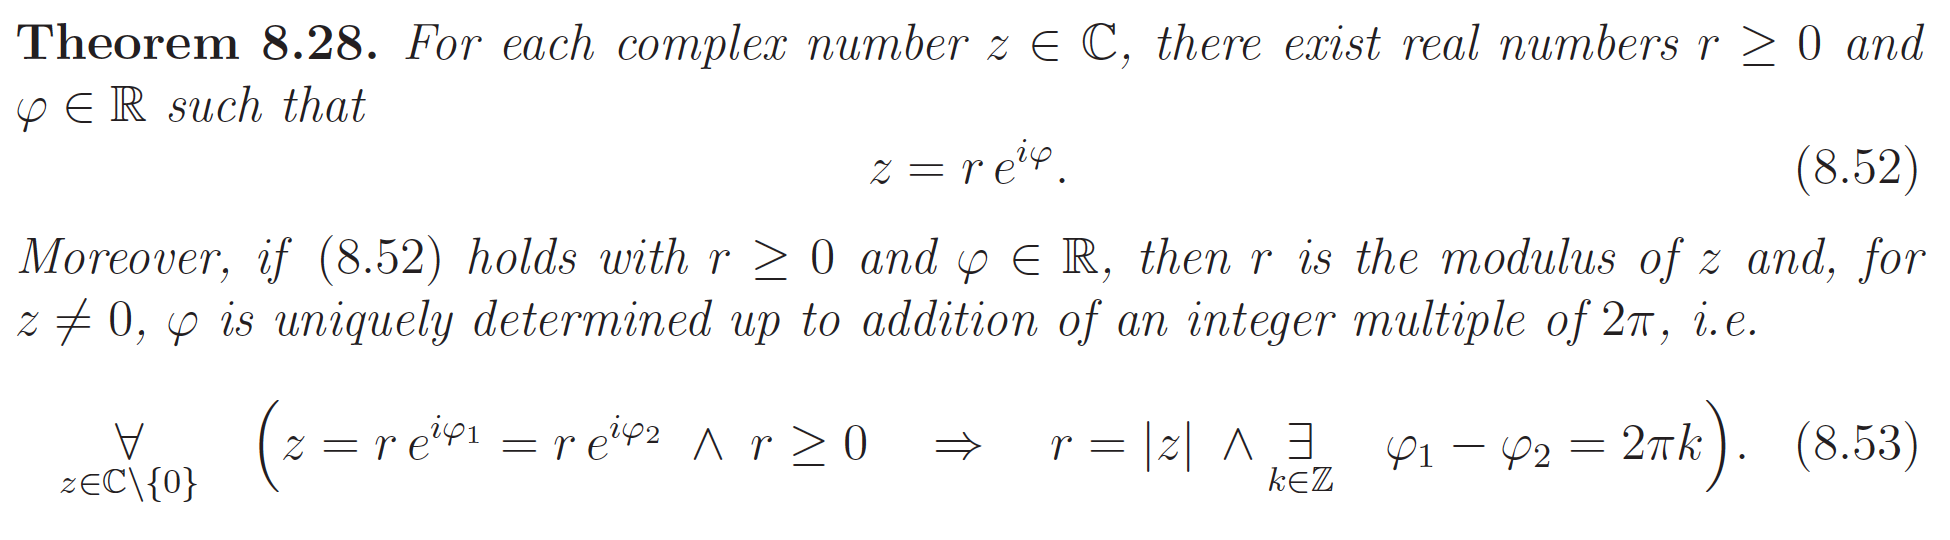
\includegraphics[width=0.7\textwidth]{media/9-5.png}
\end{figure}

\subsection{Darstellung in der komplexen Ebene (124)}
\label{Darstellung-in-der-komplexen-Ebene}

\begin{figure}[H] \centering
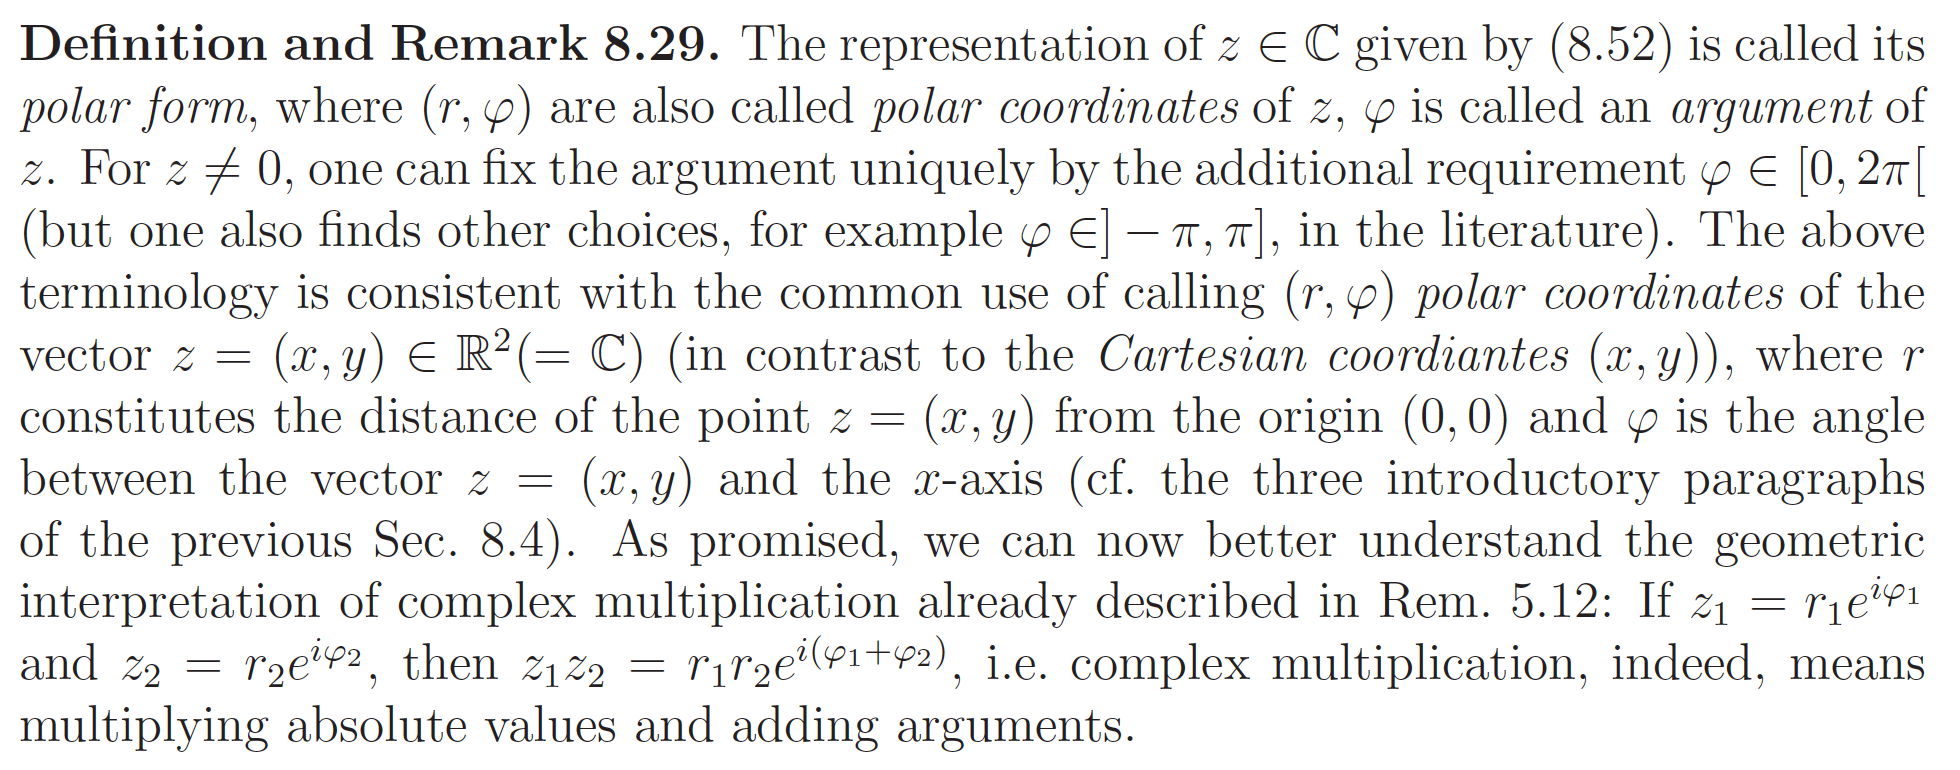
\includegraphics[width=0.7\textwidth]{media/9-6.png}
\end{figure}
\begin{figure}[H] \centering
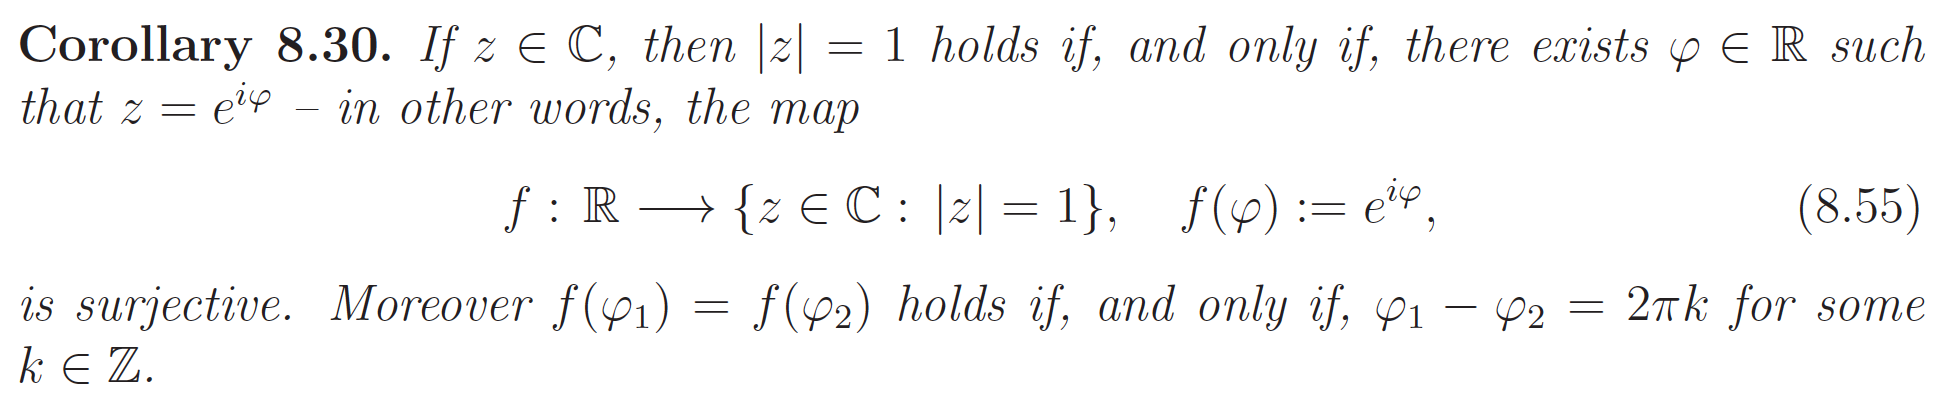
\includegraphics[width=0.7\textwidth]{media/9-6-2.png}
\end{figure}
\begin{figure}[H] \centering
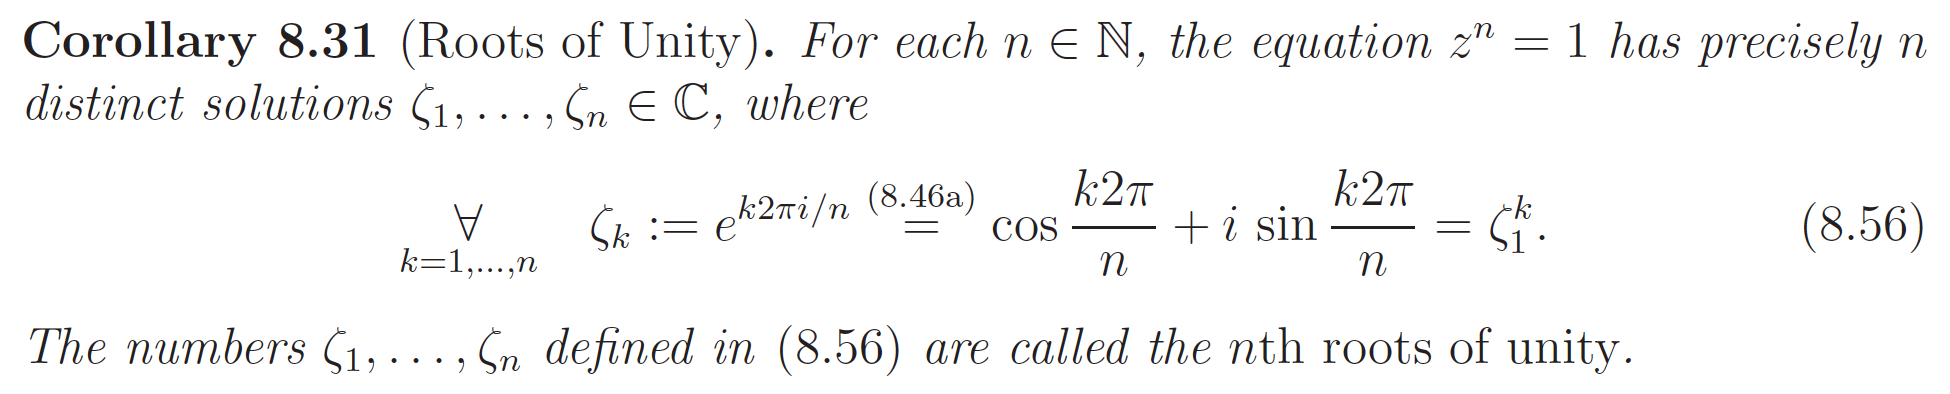
\includegraphics[width=0.7\textwidth]{media/9-6-3.png}
\end{figure}

\subsection{Multiplikation komplexer Zahlen in Polarkoordinaten (124)}

See \autoref{Darstellung-in-der-komplexen-Ebene}